\documentclass[a4paper,12pt]{article}
\usepackage[english]{babel}
\usepackage[utf8]{inputenc}
\usepackage{graphicx}
\usepackage[titletoc]{appendix}
\usepackage{amsmath}
\usepackage{epstopdf}
\usepackage{pdfpages}
\usepackage{xparse}
\usepackage{kantlipsum}
\usepackage{subcaption}
\usepackage{float}
\usepackage{titlesec}
\usepackage{listings}
\usepackage{courier}
\usepackage{enumitem}
\lstset{basicstyle=\footnotesize\ttfamily,breaklines=true}
\graphicspath{ {./images/} }
\usepackage[utf8]{inputenc}
\usepackage[T1]{fontenc}
\usepackage{times}
\usepackage{ifthen}
\usepackage[margin=25mm]{geometry}
\usepackage{fancyhdr}
\pagestyle{fancy}
\setlength{\parindent}{0pt}
\setlength{\parskip}{1ex plus 0.5ex minus 0.2ex}
\newcommand{\twodigit}[1]{\ifthenelse{#1<10}{0}{}{#1}}
\newcommand{\dagensdatum}{\number\year-\twodigit{\number\month}-\twodigit{\number\day}}

%% ------------------------------------------
% NYBILD
% Skapar centrerad bild med caption
%
% #1: Filens url relativt '/images/'
% #2: Caption
% #3: Label
% #4: Skalning
%% ------------------------------------------
\newcommand{\nyBild}[4]{
    \begin{figure}[H]
        \centering
        \includegraphics[angle=0,scale=#4]{images/#1}
        \caption{#2}
        \label{fig:#3}
    \end{figure}
}

%%  Redefinitions of commands containing @
\makeatletter
\makeatother

\newcommand{\LIPStitelsida}{
    {\ }\vspace{45mm}
    \begin{center}
        \textbf{\Huge \LIPSdokumenttyp}
    \end{center}
    \begin{center}
        {\large Alexander Vevstad, Amanda Aasa, Amanda Svennblad, \\Daniel Thomas, Lina Larsson, Olav Berg}
    \end{center}
    \begin{center}
        {\large \textbf{Version \LIPSversion}}
    \end{center}
    \begin{center}
        {Parts of chapter \ref{ch:intro} and \ref{ch:install} are based on the 2019 user guide for ENVISIoN.}
    \end{center}
    \vfill
    \begin{center}{
        \large Status}\\[1.5ex]
        \begin{tabular}{|*{3}{p{40mm}|}}
            \hline
            Granskad & \LIPSgranskare & \LIPSgranskatdatum \\
            \hline
            Godkänd & \LIPSgodkannare & \LIPSgodkantdatum \\
            \hline
        \end{tabular}
    \end{center}
}


\newenvironment{LIPSdokumenthistorik}{
    \begin{center}
        Document history\\[1ex]
        \begin{small}
            \begin{tabular}{|l|l|p{60mm}|l|l|}
                \hline
                \textbf{Version} & \textbf{Date} & \textbf{Changes} &
                \textbf{Done by} & \textbf{Reviewed} \\
                }
                {
                \hline
            \end{tabular}
        \end{small}
    \end{center}
}


\newcommand{\LIPSversionsinfo}[5]{\hline {#1} & {#2} & {#3} & {#4} & {#5} \\}
\newcounter{LIPSkravnummer}
\newcounter{LIPSunderkravnummer}[LIPSkravnummer]

\newenvironment{LIPSkravlista}{
    \begin{tabular}{|p{25mm}|p{25mm}|p{85mm}|p{5mm}|}
        }
        {
        \hline
    \end{tabular}
}

\newenvironment{LIPSleveranslista}{
    \begin{tabular}{|p{25mm}|p{15mm}|p{70mm}|p{25mm}|p{5mm}|}
        }
        {
        \hline
    \end{tabular}
}

\newenvironment{tabellexlista}{
    \begin{tabular}{|p{25mm}|p{25mm}|p{70mm}|p{20mm}|}
        }
        {
        \hline
    \end{tabular}
}

\newenvironment{dokumentlista}{
    \begin{tabular}{|p{28mm}|p{17mm}|p{39mm}|p{28mm}|p{28mm}|}
        }
        {
        \hline
    \end{tabular}
}

\newcommand{\dokumenttext}[5]{
    \hline 
    {#1} & {#2} & {#3} & {#4} & {#5} \\
}


\newcommand{\LIPSkrav}[3]{
    \hline
    \stepcounter{LIPSkravnummer}
    \textbf{Krav nr \arabic{LIPSkravnummer}} & \textbf{{#1}} & {#2} & \textbf{{#3}} \\
}

\newcommand{\tabellex}[3]{
    \hline
    Krav nr x & {#1} & {#2} & {#3} \\
}

\newcommand{\LIPSleverans}[2]{
  {#1} & {#2} & \hline
}

\newcommand{\LIPSunderkrav}[3]{
    \hline\stepcounter{LIPSunderkravnummer}\textbf{Krav nr \arabic{LIPSkravnummer}\Alph{LIPSunderkravnummer}} & \textbf{{#1}} & {#2} & \textbf{{#3}} \\
}

\newenvironment{LIPSprojektidentitet}{%
{\ }\vspace{45mm}
\begin{center}
  {\Large PROJECT IDENTITY}\\[0.5ex]
  {\small
  \LIPSartaltermin, \LIPSprojektgrupp\\
  Faculty of Science and Engineering, Linköping University, IFM
  }
\end{center}
\begin{center}
  {\small Group members}\\
%  \begin{tabular}{|p{30mm}|p{40mm}|p{35mm}|p{45mm}|}
  \begin{tabular}{|l|p{45mm}|p{25mm}|l|}
    \hline
    \textbf{Name} & \textbf{Role} & \textbf{Phone nr.} & \textbf{E-mail} \\
    \hline
}%
{%
    \hline
  \end{tabular}
\end{center}
\begin{center}
  {\small
    \textbf{Website}: \LIPSgrupphemsida\\[1ex]
    \textbf{Client}: \LIPSkund\\
    \textbf{Contact person of client}: \LIPSkundkontakt\\
    \textbf{Course examintor}: \LIPSkursansvarig\\
    \textbf{Main supervisor}: \LIPShandledare\\
  }
\end{center}
\newpage
}
\newcommand{\LIPSgruppmedlem}[4]{\hline {#1} & {#2} & {#3} & {#4} \\}

\NewDocumentCommand\secpdf{somO{1}m}{
  \clearpage
  \thispagestyle{fancy}
  \addcontentsline{toc}{section}{#3}
  \includepdf[
    pages=#4,
    pagecommand={
      \IfBooleanTF{#1}{
        \section*{#3}}{
        \IfNoValueTF{#2}{
          \section{#3}}{
          \section[#2]{#3}}}},
    scale=.80
    ]
    {#5}
}

\newenvironment{LIPSlicens}{
    \begin{center}
    \large{Licens}
    \end{center}
}{}


\usepackage{fancyhdr}
\pagestyle{fancy}
\newcommand{\LIPSdokumenttyp}{USER GUIDE}
\newcommand{\LIPSprojektgrupp}{}
\newcommand{\LIPSversion}{1.0}
\newcommand{\LIPSdatum}{\dagensdatum}
\newcommand{\LIPSartaltermin}{2019/Spring}
\newcommand{\LIPSkursnamn}{TFYA75}
\newcommand{\LIPSprojekttitel}{Visualization of electron structures}
\newcommand{\LIPSgranskare}{}
\newcommand{\LIPSgranskatdatum}{}
\newcommand{\LIPSgodkannare}{}
\newcommand{\LIPSgodkantdatum}{}

\lhead{}
\chead{\textbf{\LIPSprojekttitel}}
\rhead{\textbf{\textsl{LiTH}}\\\textbf{\dagensdatum}}
\lfoot{\textbf{User guide}}
\cfoot{\textbf{\thepage}}
\rfoot{\textbf{\LIPSkursnamn}}

\setlength{\parindent}{0pt}
\setlength{\parskip}{1ex plus 0.5ex minus 0.2ex}

\begin{document}
    \pagenumbering{gobble}
    \LIPStitelsida
    \newpage
    \pagenumbering{roman}
    \newcommand{\LIPSgruppepost}{finns ej}
\newcommand{\LIPSgrupphemsida}{https://liuonline.sharepoint.com/sites/TFYA75/TFYA75\_2019VT\_7Z/62340}

\newcommand{\LIPSdokumentansvarig}{Abdullatif Ismail}
\newcommand{\LIPSkund}{Rickard Armiento, IFM, Linköpings universitet, 581\ 83 Linköping}
\newcommand{\LIPSkundkontakt}{Rickard Armiento, rickard.armiento@liu.se}
\newcommand{\LIPSkursansvarig}{Per Sandström, per.sandstrom@liu.se}
\newcommand{\LIPShandledare}{Johan Jönsson, johan.jonsson@liu.se}

%% Argument till \LIPSgruppmedlem: namn, roll i gruppen, telefonnummer, epost
\begin{LIPSprojektidentitet}
  \LIPSgruppmedlem{Linda Le}{Project leader (PL)}{076-2249926}{linle336@student.liu.se}
  \LIPSgruppmedlem{\LIPSdokumentansvarig}{Document manager(DOK)}{072-0355455}{abdis077@student.liu.se}
  \LIPSgruppmedlem{Anton Hjert}{Anton Hjert (AH)}{070-5728891}{anthj975@student.liu.se}
  \LIPSgruppmedlem{Jesper Ericsson}{Jesper Ericsson (JE)}{070-8772630}{jeser991@student.liu.se}
  \LIPSgruppmedlem{Lloyd Kizito}{Lloyd Kizito (LK)}{070-8230589}{lloki004@student.liu.se}
\end{LIPSprojektidentitet}
    \newpage
    \tableofcontents{}
    \newpage
    %% Argument till \LIPSversionsinfo: versionsnummer, datum, ändringar, utfört av, granskat av
\addcontentsline{toc}{section}{Document history}
\begin{LIPSdokumenthistorik}
  \LIPSversionsinfo{0.1}{2019-05-21}{First draft.}{DOK, AH, JE}{Projektgruppen}
  \LIPSversionsinfo{1.0}{2019-05-25}{Second draft. Rewritten based on comments from the client.}{DOK, AH, JE}{}
\end{LIPSdokumenthistorik}
    \newpage
    \addcontentsline{toc}{section}{Licens}
\begin{LIPSlicens}
    2019 års modifikationer av den tekniska dokumentationen är licensierade under BSD, se bilaga~\ref{ref:licens}. 
\end{LIPSlicens}

    \newpage
    \pagenumbering{arabic}
    \section{Introduction}
\label{ch:intro}
ENVISIoN is an open source toolkit for electron visualization, developed as a part of the course TFYA75: Applied Physics - Bachelor's Project, given at Linköping University, LiU. It's implemented by using a modified verision of the Inviwo visualization framework, developed at the Scientific Visualization Group at Linköping University, LiU.

The present version was developed during the spring semester of 2021 by a project group consisting of: Gabriel Anderberg, Adam Engman, Joakim Stenborg, Kristoffer Gubberud Maras and Didrik Axén. The Supervisor was Marian Brännvall, the Requisitioner and co-supervisor was Rickard Armiento and the Visualisation expert was Peter Steneteg. The Course examiner was Per Sandström. The work is based on a previous version by the project group taking the course in the spring semester of 2020 consisting of: Alexander Vevstad, Amanda Aasa, Amanda Svennblad, Daniel Thomas, Lina Larsson and Olav Berg, with the Supervisor Joel Davidsson, the Requisitioner and co-supervisor Rickard Armiento, the Visualisation expert Peter Steneteg and the Course examiner Per Sandström. That work was based on a previous version by the project group taking the course in the spring semester of 2019 consisting of: Linda Le, Abdullatif Ismail, Anton Hjert, Lloyd Kizito and Jesper Ericsson, with the Supervisor Johan Jönsson, the Requisitioner and co-supervisor Rickard Armiento, the Visualisation expert Peter Steneteg and the Course examiner Per Sandström. That work was based on a previous version by the project group taking the course in the spring semester of 2018 consisting of: Anders Rehult, Marian Brännvall, Andreas Kempe and Viktor Bernholtz with the Supervisor Johan Jönsson, the Requisitioner and co-supervisor Rickard Armiento, the Visualisation expert Rickard Englund and Course examiner Per Sandström. That work was is based on the work by the project group taking the course in the spring term of 2017 consisting of: Josef Adamsson, Robert Cranston, David Hartman, Denise Härnström and Fredrik Segerhammar. Supervisor: Johan Jönsson; Requisitioner and co-supervisor: Rickard Armiento; Visualization expert: Peter Steneteg; and Course examiner: Per Sandström.
\\\\
ENVISIoN provides a graphical user interface and a set of Python scripts that allow the user to:
\begin{itemize}
    \item Read and parse output from electronic structure calculations made by the program VASP and storing the result in a structured HDF5 file.
    
    \item Generate Inviwo visualizations for common tasks when analyzing electronic structure calculations. Presently there is support for visualizing the crystal structure of the unit cell of a material, electron localization function (ELF)-data, electronic charge density, electronic band structure, radial Distribution Function and density of states - both total and partial, forces on atoms as well as molecular dynamics. The system also provides the ability to interconnect some of the networks mentioned above.
\end{itemize}
    \newpage
    \section{How to build Inviwo with ENVISIoN on Ubuntu
18.04 LTS}

\label{ch:install}
These instructions show how to build Inviwo and ENVISIoN on Ubuntu
18.04 LTS.

\subsection{Install git}
Start by installing git, which will be used to fetch ENVISIoN in the
next step.
\begin{lstlisting}[frame = single, breaklines=true]
    sudo apt install git
\end{lstlisting}

\subsection{Download ENVISIoN}
Go to your home folder and clone ENVISIoN from Github. This guide will
assume that both ENVISIoN and Inviwo will be placed directly under the
home folder.
\begin{lstlisting}[frame = single, breaklines=true]
    cd
    git clone https://github.com/rartino/ENVISIoN
\end{lstlisting}

\subsection{Prepare Inviwo using the ENVISIoN install script}
ENVISIoN provides an install script for Ubuntu 18.04 LTS. Executing
the installation script will install all required dependencies, clone
Inviwo from Github and configure the Inviwo build.

The script should \emph{NOT} be run as root, but as your own user and
it will ask for your password when it needs root rights. It is
possible that the script will ask for other user input during the
process, if that's the case, just accept the default.
\begin{lstlisting}[frame = single, breaklines = true]
    cd ~/ENVISIoN/scripts
    ./install.sh /home/$USER/ENVISIoN /home/$USER/inviwo
\end{lstlisting}

Once the installation script has run, it prints build instructions.
Follow the instructions and start the build. The instructions will
tell you to \emph{cd} to the build directory and execute make.

An easy way to modify the build settings, if needed, is to install
the cmake curses gui and run it in the build directory.

To install the cmake gui:
\begin{lstlisting}[frame = single, breaklines = true]
    sudo apt install cmake-curses-gui
\end{lstlisting}

Running cmake in the build directory:
\begin{lstlisting}[frame = single, breaklines = true]
    cd ~/inviwo/build
    ccmake .
\end{lstlisting}

When in the GUI, press \emph{c} to apply the current configuration,
\emph{g} to generate build files and \emph{q} to quit. If settings
have changed, it is possible that you will need to press \emph{c} more
than once before the \emph{g} option becomes available.

After having generated the build files, the project can now be rebuilt
with the new settings by executing \emph{make} like earlier.
    \newpage
    \section{How to build Inviwo with ENVISIoN on other OS}

\subsection{Install git}
Start by installing git, which will be used to fetch ENVISIoN in the next step. Git can be downloaded from the website below.
\begin{lstlisting}[frame = single, breaklines=true]
    https://git-scm.com/downloads
\end{lstlisting}

\subsection{Download ENVISIoN}
Change the working directory to the home folder and clone ENVISIoN from Github. This guide will assume that both ENVISIoN and Inviwo will be placed directly under the home folder. Clone the ENVISIoN repository be executing the command below.
\begin{lstlisting}[frame = single, breaklines=true]
    git clone https://github.com/rartino/ENVISIoN
\end{lstlisting}

\subsection{Prepare Inviwo for build}
To be able to install Inviwo, all required dependencies needs to installed: 
\begin{itemize}
    \setlength\itemsep{0em}
    \item gcc
    \item hdf5 
    \item cmake
    \item qt
    \item python3
    \item numpy
    \item h5py
    \item regex
    \item wxPython
    \item pybind11
\end{itemize}

Make sure to install the latest version of all the softwares mentioned above. Clone the Inviwo repository into the home folder and make it your working directory. Clone the Inviwo repository be executing the command below.

\begin{lstlisting}[frame = single, breaklines = true]
    git clone https://github.com/inviwo/inviwo.git
\end{lstlisting}

ENVISIoN isn't compatible with the newest version of Inviwo due to a reconstruction in the Inviwo file system on April 15, 2019. To make ENVISIoN compatible with Inviwo that just got cloned, a checkout of a compatible version is needed.

\begin{lstlisting}[frame = single, breaklines = true]
    git checkout d20199dfd37c80559ce687243d296f6ce3e41c71
\end{lstlisting}

Some minor alterations has been made on the Inviwo source code by the ENVISIoN project group that need to be patched. 

\begin{lstlisting}[frame = single, breaklines = true]
    git apply < "~/ENVISIoN/inviwo/patches/2019/envisionTransferFuncFix2019.patch"
    git apply < "~/ENVISIoN/inviwo/patches/2019/paneProperty2019.patch"
\end{lstlisting}

The only remaining change in the Inviwo repository is an update of its submodules.
 
\begin{lstlisting}[frame = single, breaklines = true]
    git submodule init
\end{lstlisting}

Create a build directory in the home folder and configure the ENVISIoN module and project path using cmake. Execute the command below when standing in the build directory. 

\begin{lstlisting}[frame = single, breaklines = true]
    cmake .. -DIVW_EXTERNAL_PROJECTS="~/ENVISIoN/inviwo/app" \
         -DIVW_EXTERNAL_MODULES="$~/ENVISIoN/inviwo/modules" \
         -DIVW_MODULE_CRYSTALVISUALIZATION=ON \
         -DIVW_MODULE_FERMI=OFF \
         -DIVW_MODULE_GRAPH2D=ON \
         -DIVW_MODULE_PYTHON3=ON \
         -DIVW_MODULE_PYTHON3QT=ON \
         -DIVW_MODULE_QTWIDGETS=ON \
         -DIVW_MODULE_HDF5=ON
\end{lstlisting}

Inviwo is now ready to be installed with the ENVISIoN modules added. Add the \emph{-j} extension to use multiple cores while installing.
\begin{lstlisting}[frame = single, breaklines = true]
    make -j5
\end{lstlisting}
    \section{Start ENVISIoN or Inviwo}
\label{sec: start envision}
\subsection{Start ENVISIoN}
When the building for Inviwo with ENVISIoN is finished, we can start the application's graphical user interface. If you have structured the file system as explained in section 2 and section 3, the start up of the application should be the same on every operating system. Open up a terminal or command window and execute the following command in the terminal:

\begin{lstlisting}[frame = single, breaklines = true]
    python3 ~/ENVISIoN/ENVISIoN/envisionGUI/GUI.py
\end{lstlisting}

The application ENVISIoN should start and the GUI will pop up. For further instruction concering ENVISIoN's GUI, see section \ref{sec:newGUI}.

\subsection{Start Inviwo}
During the development of ENVISIoN it can be an advantage to use only Inviwo and its graphical user interface. If the installation of ENVISIoN with Inviwo is made correctly, open a terminal or command window and navigate to the ENVISIoN directory: 

\begin{lstlisting}[frame = single, breaklines = true]
    cd ~ENVISIoN/ENVISIoN
\end{lstlisting}

Then, type in the following command in the terminal to start Inviwo:

\begin{lstlisting}[frame = single, breaklines = true]
    inviwo-build/bin/inviwo
\end{lstlisting}
    \newpage
    \section{Start Inviwo and run ENVISIoN scripts}

\\
If the user wishes to run Inviwo with its own graphical user interface, it's possible and still have access to the visualizations provided by ENVISIoN. These visualizations are stored in the form of Python scripts that can be compiled through the Inviwo user interface.

To run Inviwo in an UNIX environment, execute the commands below.

\begin{lstlisting}[frame = single, breaklines=true]
    cd ~/ENVISIoN/ENVISIoN
    inviwo-build/bin/inviwo
\end{lstlisting}

When the Inviwo interface has opened, follow the instructions given in figure \ref{fig:Inviwo} and in the list below to run a visualization script.

\begin{enumerate}
\item Locate and press the Python menu in the Inviwo bar.
\item Open the Python editor by pressing it.
\item In the Python editor, click Open Script.
\item Select one of the scripts. The ENVISIoN scripts can be located in \emph{$\sim$/ENVISIoN/demo}.
\item Click open.
\item Click the button in the top left corner to run.
\end{enumerate}

\begin{figure}[ht]
    \centering
    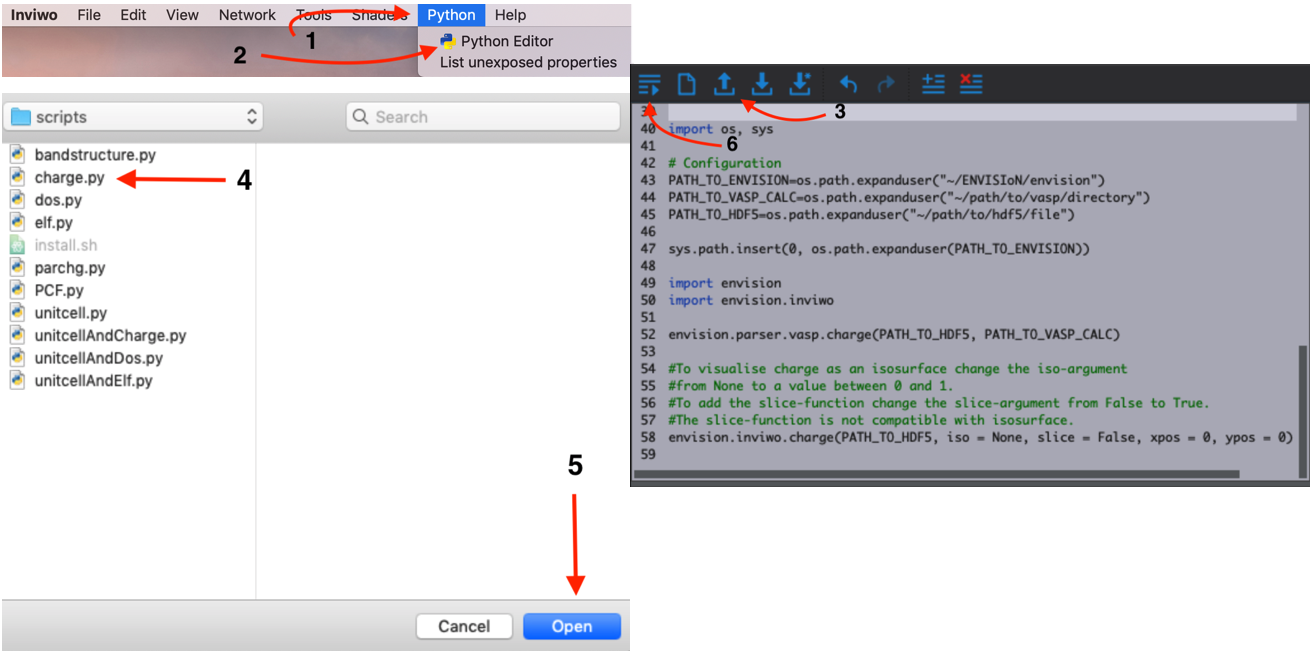
\includegraphics[angle=0, width=\linewidth]{Images/completeInviwo.png}
    \caption{Cutout from Inviwo with instructions on how to run a ENVISIoN visualization script in numeric order.}
    \label{fig:Inviwo}
\end{figure}

    \newpage
    \section{Using Legacy GUI}
\label{sec:GUI}
ENVISIoN is equipped with a graphical user interface to simplify the usage of ENVISIoN. 

\subsection{Start-up}
When the user starts the application through a computer terminal (see chapter \ref{sec: start envision}) a window opens, see figure \ref{fig:GUIStartupUbuntu} for Ubuntu and figure for Windows. The start-up window of ENVISIoN has a sidebar menu to the left with different choices. Each choice has its own content to the right. By default, the ``Dataset loader'', is chosen from start. The other possible choices are ``Parser'' or ``About''. Under ``Active datasets'' the loaded datasets will appear. Each alternative will be explained in their own sections in this chapter. The following figures of the GUI in this chapter will be for Windows but the content is the same for every operative system.

\begin{figure}[H]
    \centering
    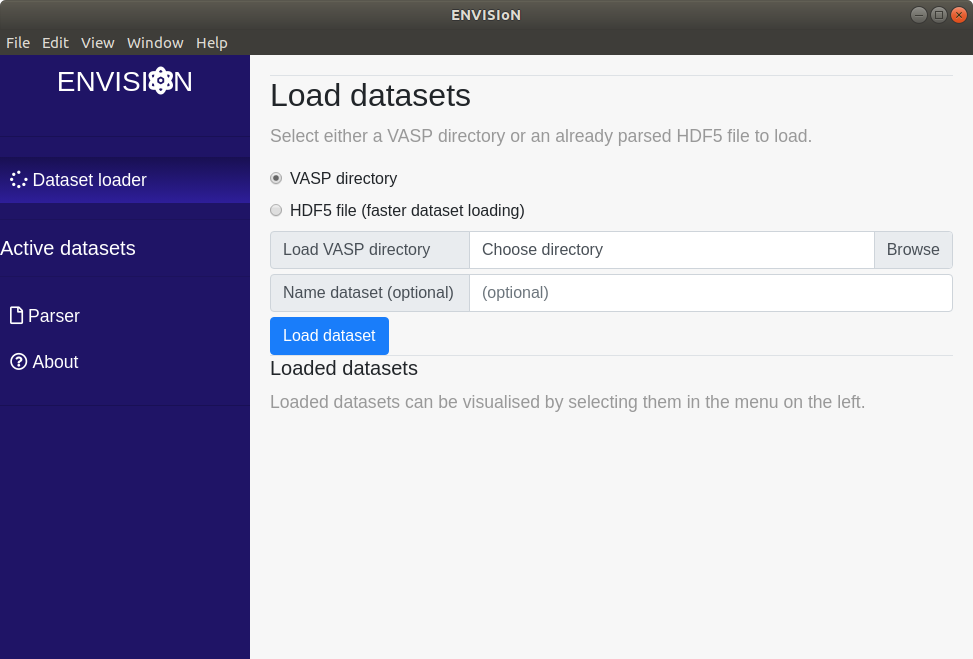
\includegraphics[scale = 0.3]{Images/GUI_start_Ubuntu.png}
    \caption{ENVISIoN start-up window for Linux.}
    \label{fig:GUIStartupUbuntu}
\end{figure}

\begin{figure}[H]
    \centering
    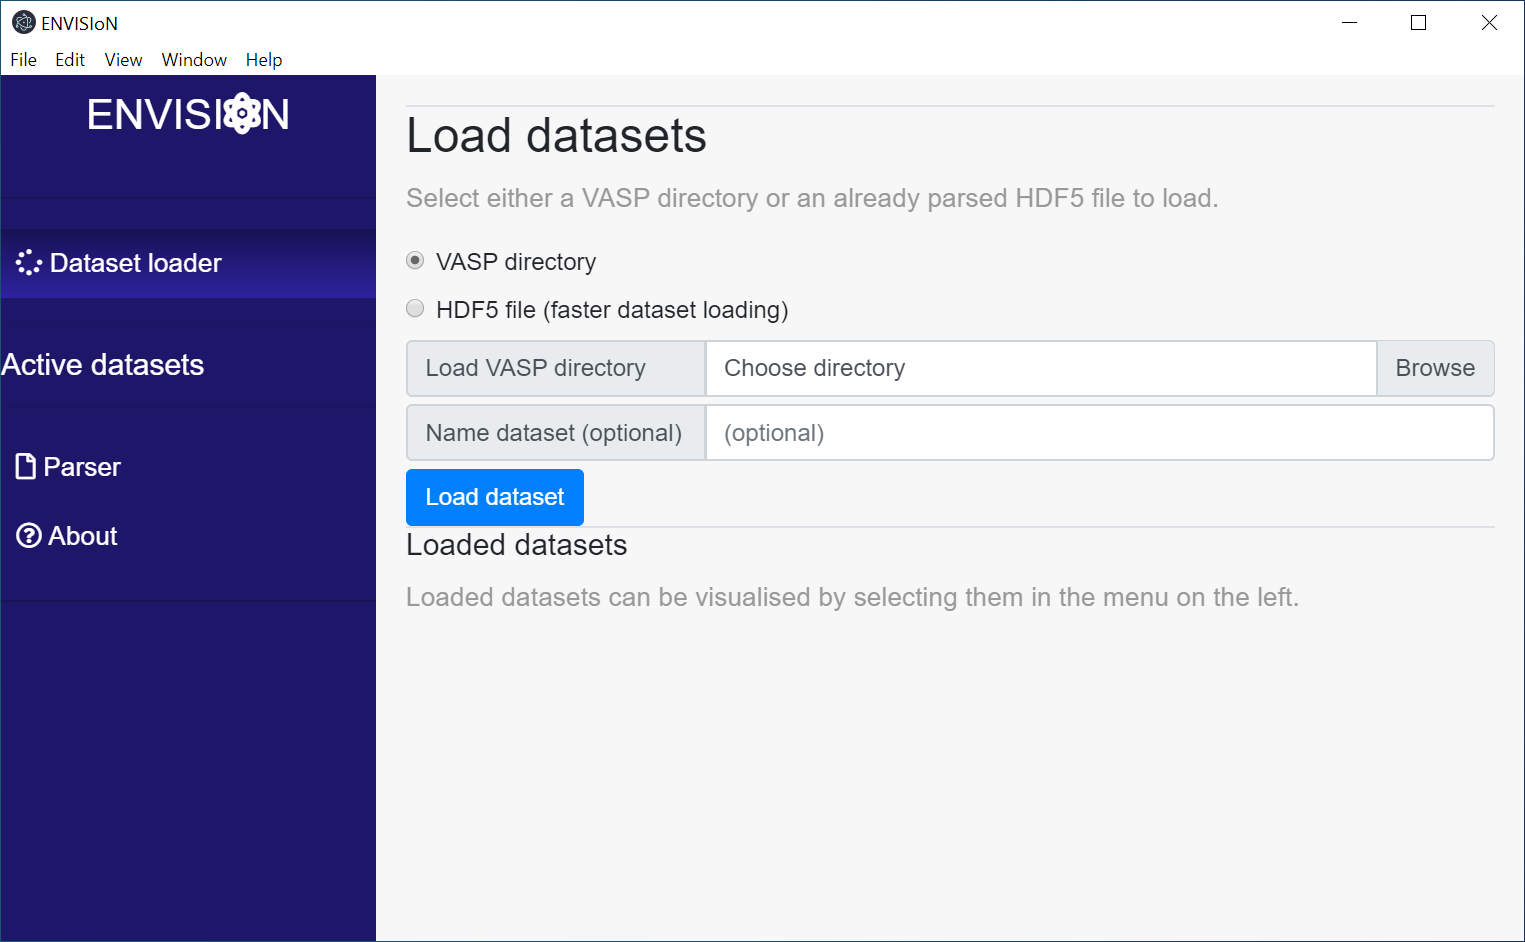
\includegraphics[scale = 0.4]{Images/GUI_start_Windows.png}
    \caption{ENVISIoN start-up window for Windows.}
    \label{fig:GUIStartupUbuntu}
\end{figure}

\subsection{Dataset loader}
In the ``Dataset loader'' a user can select either a VASP file or a HDF5 file to load which then will be visualised. To load a VASP file, the box ``VASP directory'' need to be checked. To load a HDF5 file the box ``HDF5 file'' need to be checked. 

For a quick step-by-step guide, scroll down to section \ref{sec:Dataset step-by-step}.

\subsubsection{Load a VASP file}
For loading a VASP file, the content for the ``Dataset loader'' is shown below in figure \ref{fig:GUIDatasetloaderVASP}.

\begin{figure}[H]
    \centering
    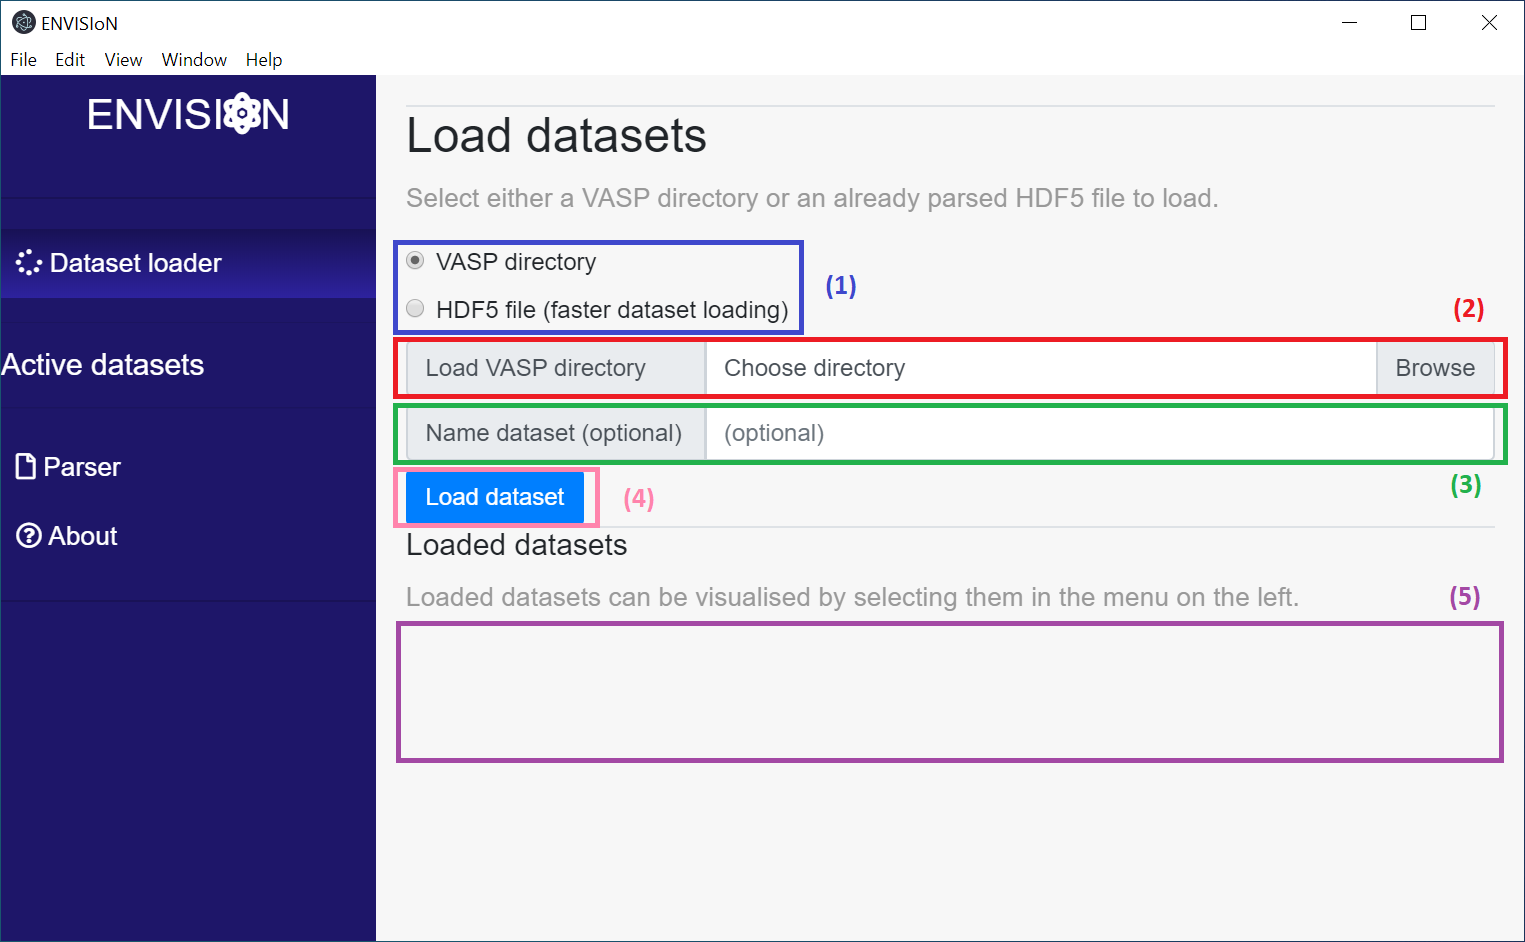
\includegraphics[scale = 0.45]{Images/GUI_Datasetloader_VASP.png}
    \caption{Dataset loader for VASP source.}
    \label{fig:GUIDatasetloaderVASP}
\end{figure}

In the blue box labeled (1) the box ``VASP directory'' need to be checked. In the red box labeled (2) the path to the VASP directory to load is selected. By clicking on ``Browse'' a new window will appear where the user navigates to the VASP directory on the computer and selects it. In the green box labeled (3) the user can write a name for the dataset. This is optional. In the pink box labeled (4) is the ``Load dataset'' button. When pressing this button the dataset will be loaded. The loaded dataset will be displayed in the purple box labeled (5) and in the sidebar menu under ``Active datasets''.

\subsubsection{Load a HDF5 file}
For loading a HDF5 file, the content for the ``Dataset loader'' is shown below in figure \ref{fig:GUIDatasetloaderHDF5}.

\begin{figure}[H]
    \centering
    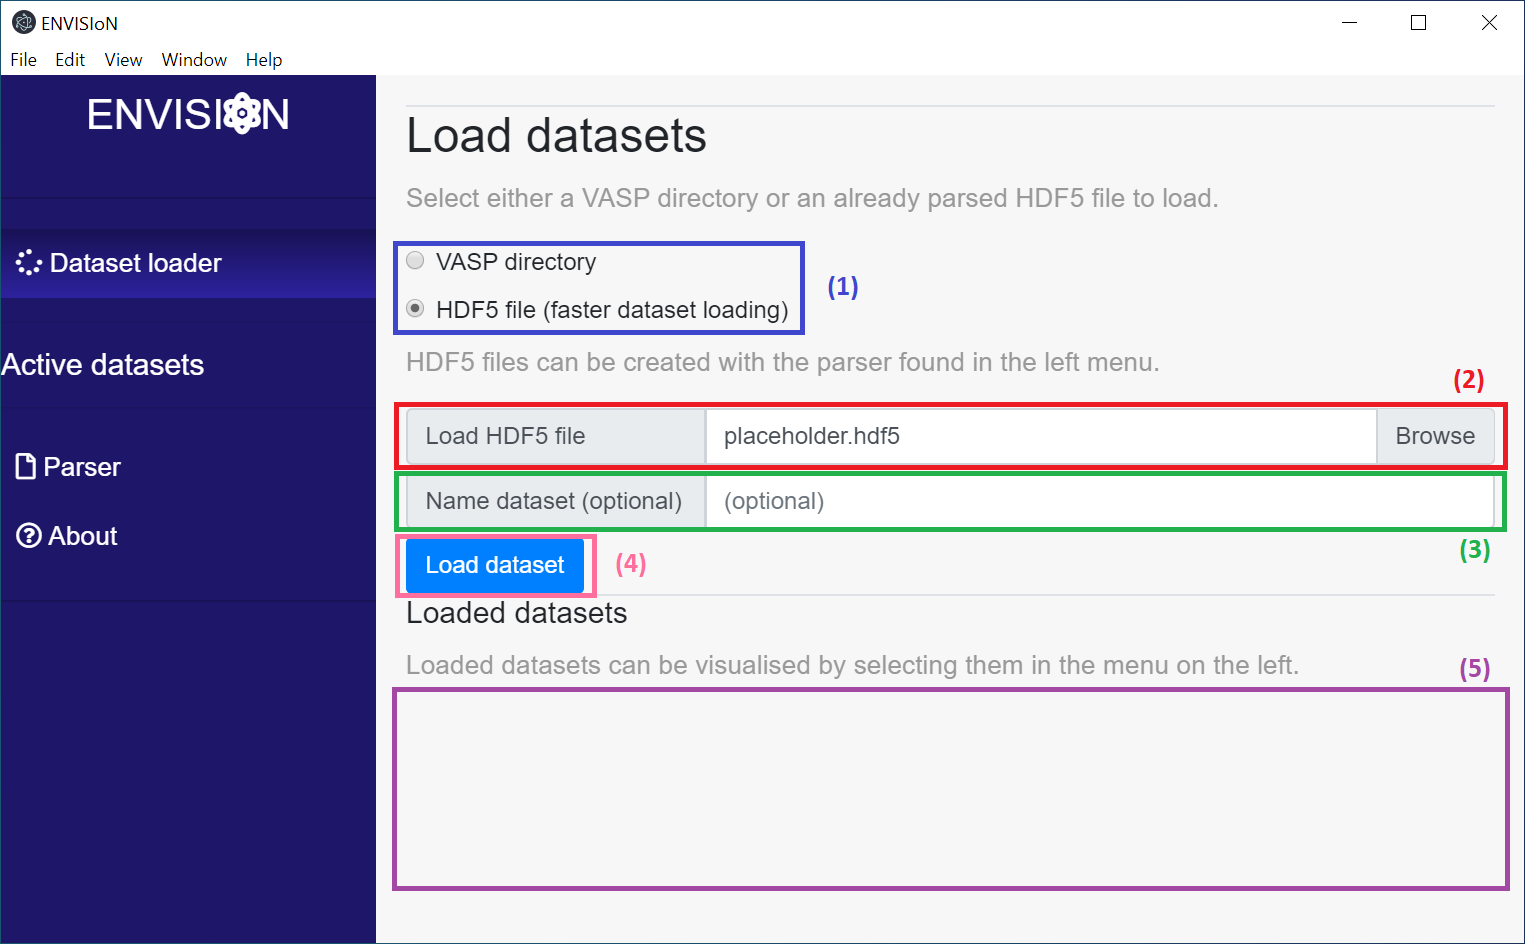
\includegraphics[scale = 0.45]{Images/GUI.Datasetloader_HDF5.png}
    \caption{Dataset loader for HDF5 source.}
    \label{fig:GUIDatasetloaderHDF5}
\end{figure}

In the blue box labeled (1) the box ``HDF5 file'' need to be checked. In the red box labeled (2) the path to the HDF5 file to load is selected. By clicking on ``Browse'' a new window will appear where the user navigates to the HDF5 file on the computer and selects it. In the green box labeled (3) the user can write a name for the dataset. This is optional. In the pink box labeled (4) is the ``Load dataset'' button. When pressing this button the dataset will be loaded. The loaded dataset will be displayed in the purple box labeled (5) and in the sidebar menu under ``Active datasets''.

\subsubsection{Quick Step-by-step guide}
\label{sec:Dataset step-by-step}
To load a VASP-file (referring to figure \ref{fig:GUIDatasetloaderVASP}):
\begin{enumerate}
    \item Check the box ``VASP directory'' in (1).
    \item Choose a VASP directory on your computer by clicking ``Browse'' in (2).
    \item (optional) Name the dataset by writing in (3).
    \item Click ``Load dataset'' in (4).
    \item Now the loaded dataset is showing in (5) and in the sidebar menu under ``Active datasets''.
\end{enumerate}

To load a HDF5 file (referring to figure \ref{fig:GUIDatasetloaderHDF5}):
\begin{enumerate}
    \item Check the box ``HDF5 file'' in (1).
    \item Choose a HDF5 file on your computer by clicking ``Browse'' in (2).
    \item (optional) Name the dataset by writing in (3).
    \item Click ``Load dataset'' in (4).
    \item Now the loaded dataset is showing in (5) and in the sidebar menu under ``Active datasets''.
\end{enumerate}

\subsection{Active datasets}
When a dataset is loaded for visualisation it will appear under ``Active datasets'' in the sidebar menu. 

\subsubsection{Starting the visualisation}
By clicking on one of datasets under ``Active datasets'', new content will show up to the right, see figure \ref{fig:GUIChosevistype} below. In figure \ref{fig:GUIChosevistype} the dataset ``BaSO4\_ORC'' is loaded as an example.

\begin{figure}[H]
    \centering
    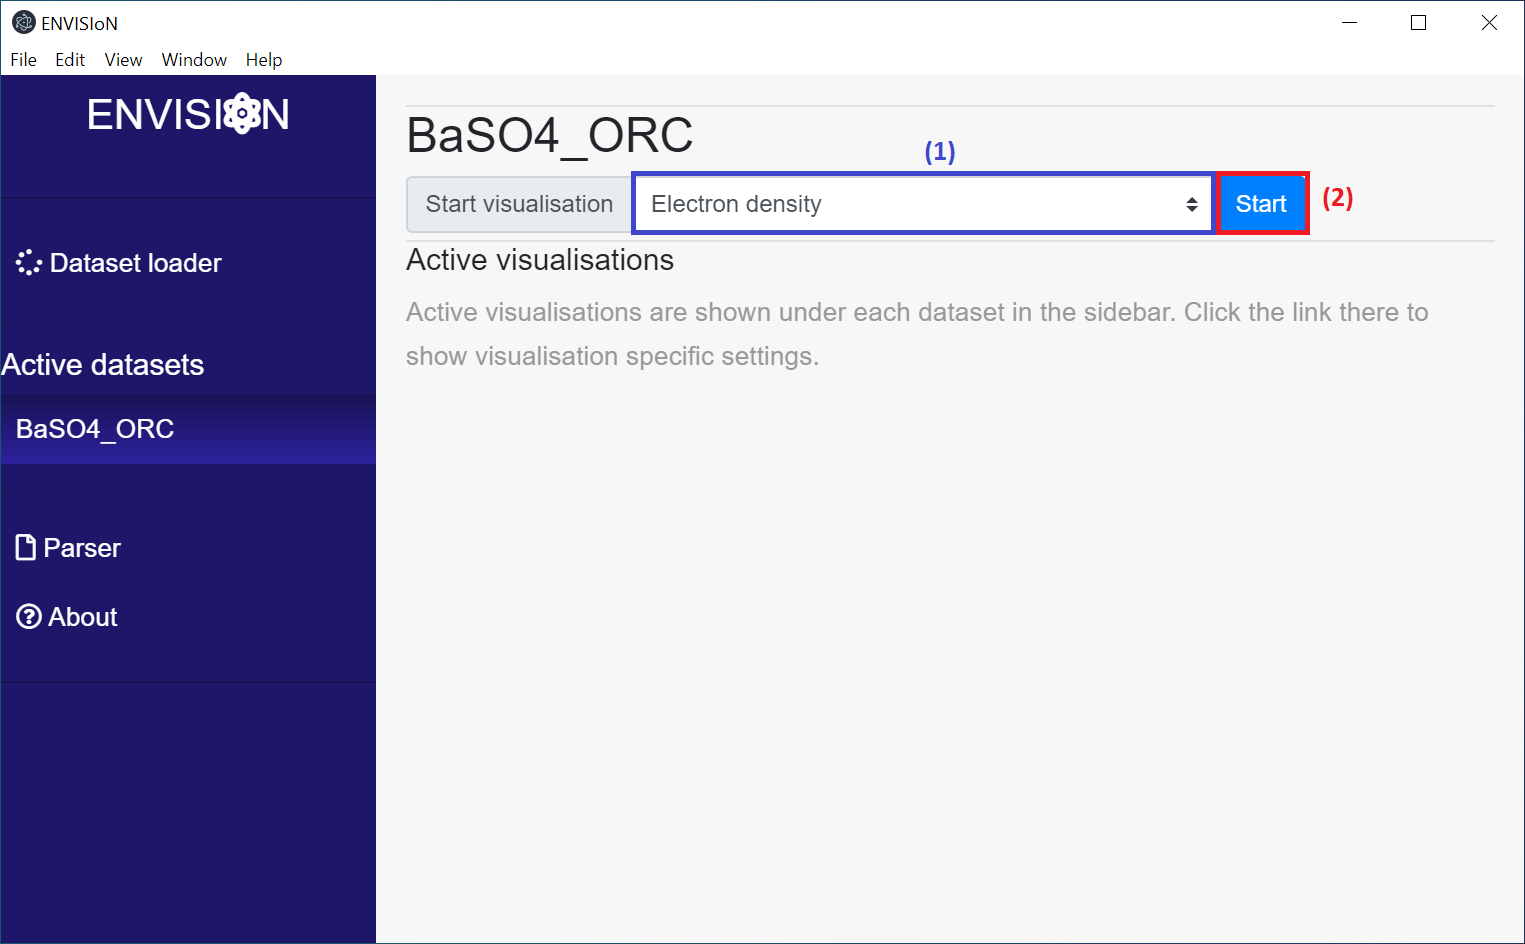
\includegraphics[scale = 0.45]{Images/GUI_Chosevistype.png}
    \caption{Start the visualisation. Here the dataset BaSO4\_ORC is loaded as an example.}
    \label{fig:GUIChosevistype}
\end{figure}

By pressing the area inside the blue box labeled (1) the user can select which visualisation type to visualise from the drop-down menu. The different possible visualisation types are: 

\begin{itemize}
    \item Electron density
    \item Unitcell
    \item Bandstructure 3D
    \item Fermi surface
\end{itemize}

In the red box labeled (2) is the ``Start'' button. When pressing this button the visualisation will start for the chosen visualisation type. The visualisation will appear under the loaded dataset in the sidebar menu. When pressing the visualisation in the sidebar menu new content with visualisation controls will appear to the right. Also the canvas/canvases belonging to the selected visualisation type will pop up next to the GUI.

\subsubsection{Visualisation controls}
When clicking on the ongoing visualisation of a dataset in the sidebar, visualisation controls will appear to the right. These controls are different for different visualisation types. There are only controls for the visualisation types ``Electron density'' and ``Fermi surface''. 

\textbf{Electron density controls}
\newline
If the ongoing visualisation is ``Electron Density'' the controls for interacting with the visualisation are shown in figure \ref{fig:GUICharge} below.

\begin{figure}[H]
    \centering
    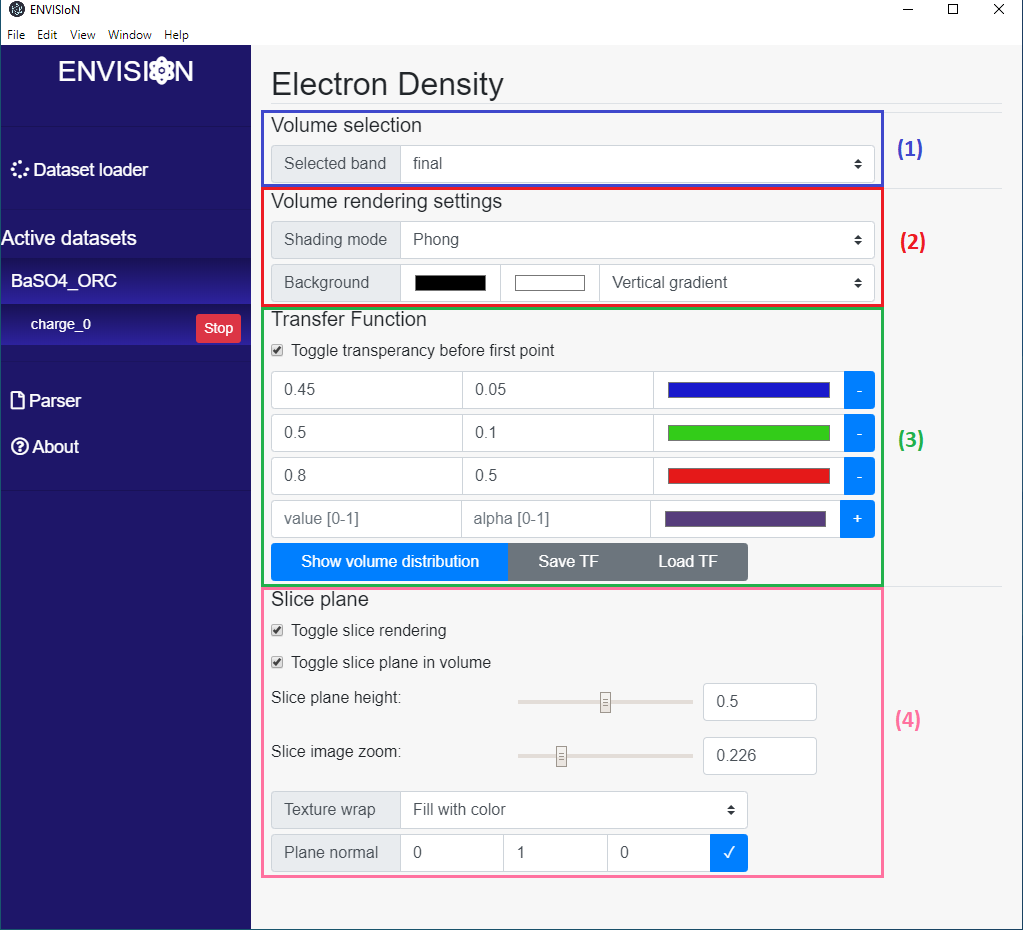
\includegraphics[scale = 0.56]{Images/GUI_Chargecontent.png}
    \caption{The content for the electron density visualisation controls.}
    \label{fig:GUICharge}
\end{figure}

For electron density the user can control the volume selection by selecting band, the volume rendering settings, the transfer function by visualising certain density intervals with different colors and the slice plane to see the electron density in a 2-dimensional plane. In the blue box labeled (1) the user can regulate the volume selection by selecting which band to visualise from a drop-down menu. In the red box labeled (2) the user can select the Shading mode from a drop-down menu and also change the Background color and gradient. In the green box labeled (3) the user can change the transfer function. This is a way to choose different colors for different electron density intervals. The intervals are normalized. The user can also select the blue ``Show volume distribution'' button and then a new diagram will pop up containing information about the volume distribution for the selected dataset. In the pink box labeled (4) the user can configure the slice plan to see a 2-dimensional cross-sectional area of the electron density connected to the 3-dimensional electron density.

\textbf{Fermi surface controls}
\newline
If the ongoing visualisation is ``Fermi surface'' the controls for interacting with the visualisation are shown in figure \ref{fig:GUIFermi} below.

\begin{figure}[H]
    \centering
    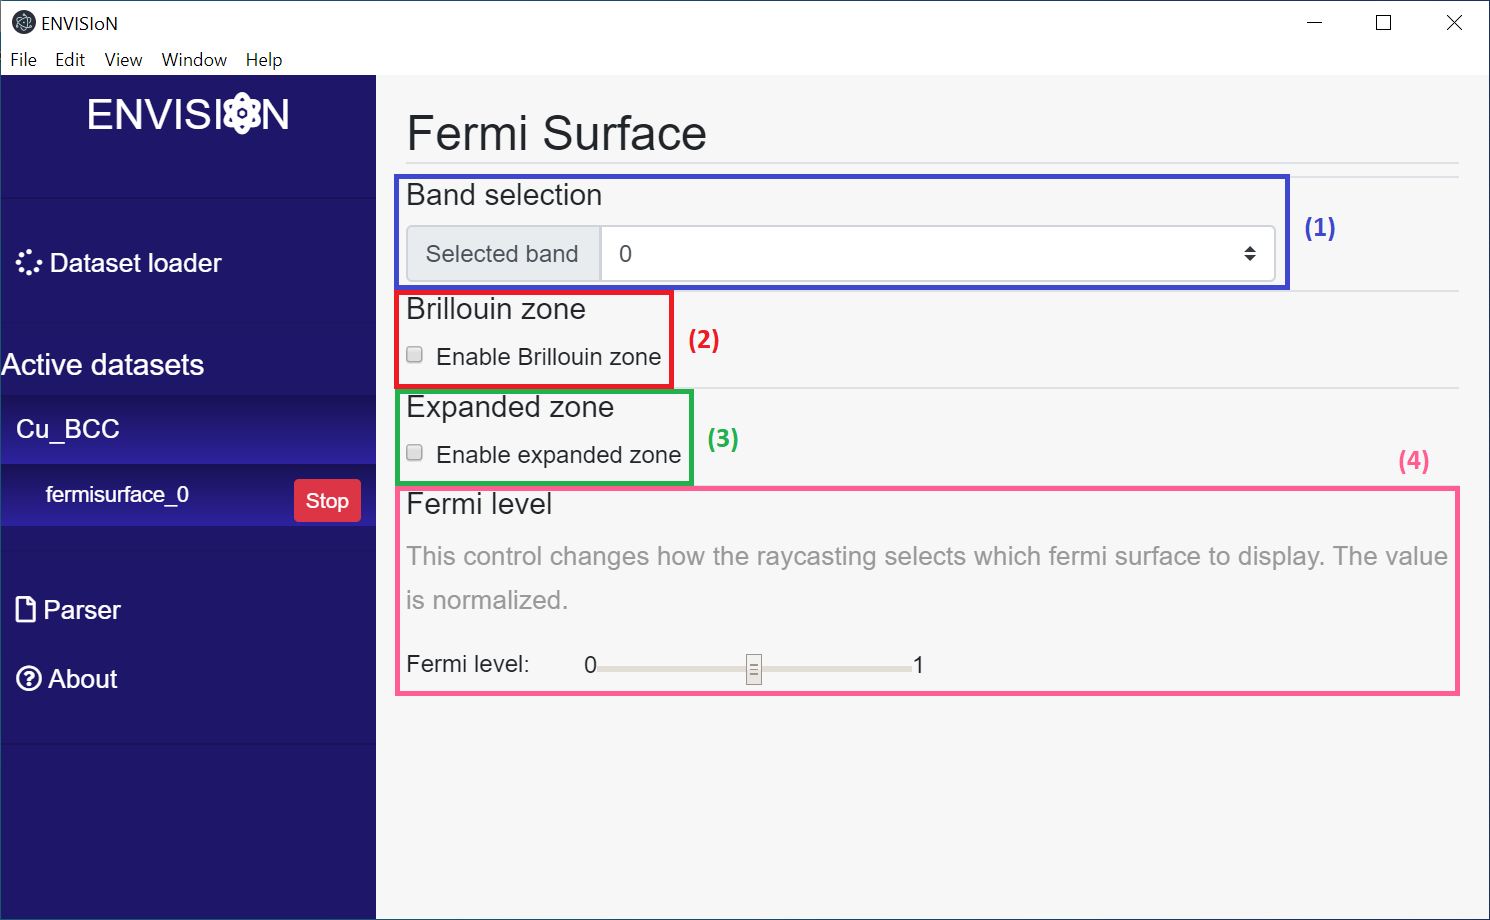
\includegraphics[scale = 0.45]{Images/GUI_Fermicontent.png}
    \caption{The content for the fermi visualisation controls.}
    \label{fig:GUIFermi}
\end{figure}

For fermi surface the user can control which band that should be visualised, enable the Brillouin zone, enable expanded zone and regulate the fermi level. In the blue box labeled (1) the user can select which band to visualise from a drop-down menu. When starting the visualisation the current band will be selected automatically and also the correct fermi level (in the pink box labeled (4)) for each band is set to default. In the red box labeled (2) the user can enable or disable the Brillouin zone by having the checkbox checked or unchecked. In the green box labeled (3) the user can enable or disable expanded zone by having the checkbox checked or unchecked. In the pink box labeled (4) the user can control the fermi level by dragging the slider to the right or to the left. The scale is normalized between 0 and 1.

\subsection{Parser}
If you choose ``Parser'' in the sidebar menu, new content will be exposed to the right, see figure \ref{fig:GUIParser} below. 

\begin{figure}[H]
    \centering
    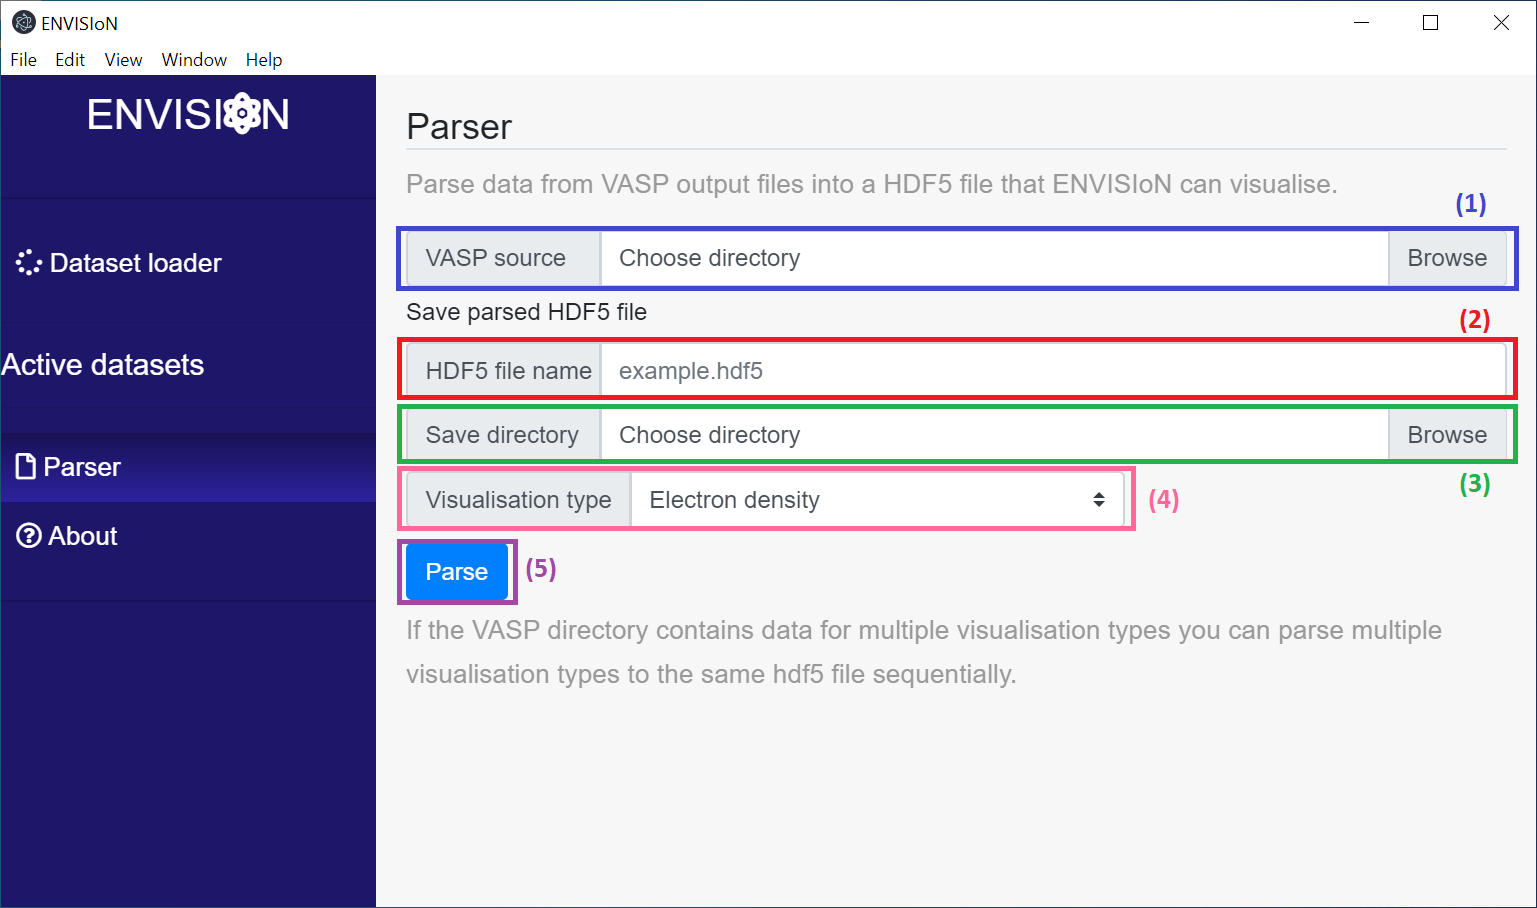
\includegraphics[scale = 0.45]{Images/GUI_Parserstart.png}
    \caption{The content for the parser menu.}
    \label{fig:GUIParser}
\end{figure}

For a quick step-by-step guide, scroll down to section \ref{sec:Parse step-by-step} 

In figure \ref{fig:GUIParser}, in the blue box labeled (1), the path to the directory of VASP files to parse is selected. By clicking on ``Browse'' a new window will appear where the user navigates to the directory of the VASP files on the computer and selects it. In the red box labeled (2) the user writes the name for the new HDF5 file, it needs to end with .hdf5. In the green box labeled (3) the path to the saving directory of the new HDF5 file is selected. When clicking on ``Browse'' a new window will appear where the user navigates to the saving directory and selects it. In the pink box labeled (4) the user can select which visualisation type to parse from a drop-down menu. The possible types to parse are:

\begin{itemize}
    \item Electron density
    \item Bandstructure
    \item Unitcell
    \item Fermi surface
\end{itemize}

In the purple box labeled (5) is the ``Parse'' button. By pressing this button the parser will parse the VASP files and create a HDF5 file in the saving directory. 

\subsubsection{Quick Step-by-step guide}
\label{sec:Parse step-by-step}
Parsing VASP files to a HDF5 file:
\begin{enumerate}
    \item Enter path to VASP directory in (1).
    \item Write name for the HDF5 file in (2).
    \item Enter path to saving directory in (3)
    \item Select type in (4).
    \item Press ``Parse'' in (5).
\end{enumerate}

\subsection{About}
When selecting ``About'' in the sidebar menu there will be new content to the right that contains brief information about ENVISIoN and the project members through the years.

\subsection{If ENVISIoN does not respond or crashes}
If the user have multiple ongoing visualisation or if the user has stopped one visualisation and then want to start another the GUI can stop responding or sometimes even crash. If the GUI falls behind in the number of requests from the user, it will stop responding and a pop up in the GUI will show. The pop up contains the message ``Loading... envision is # requests behind''. See figure \ref{fig:GUINotresponding} below. 

\begin{figure}[H]
    \centering
    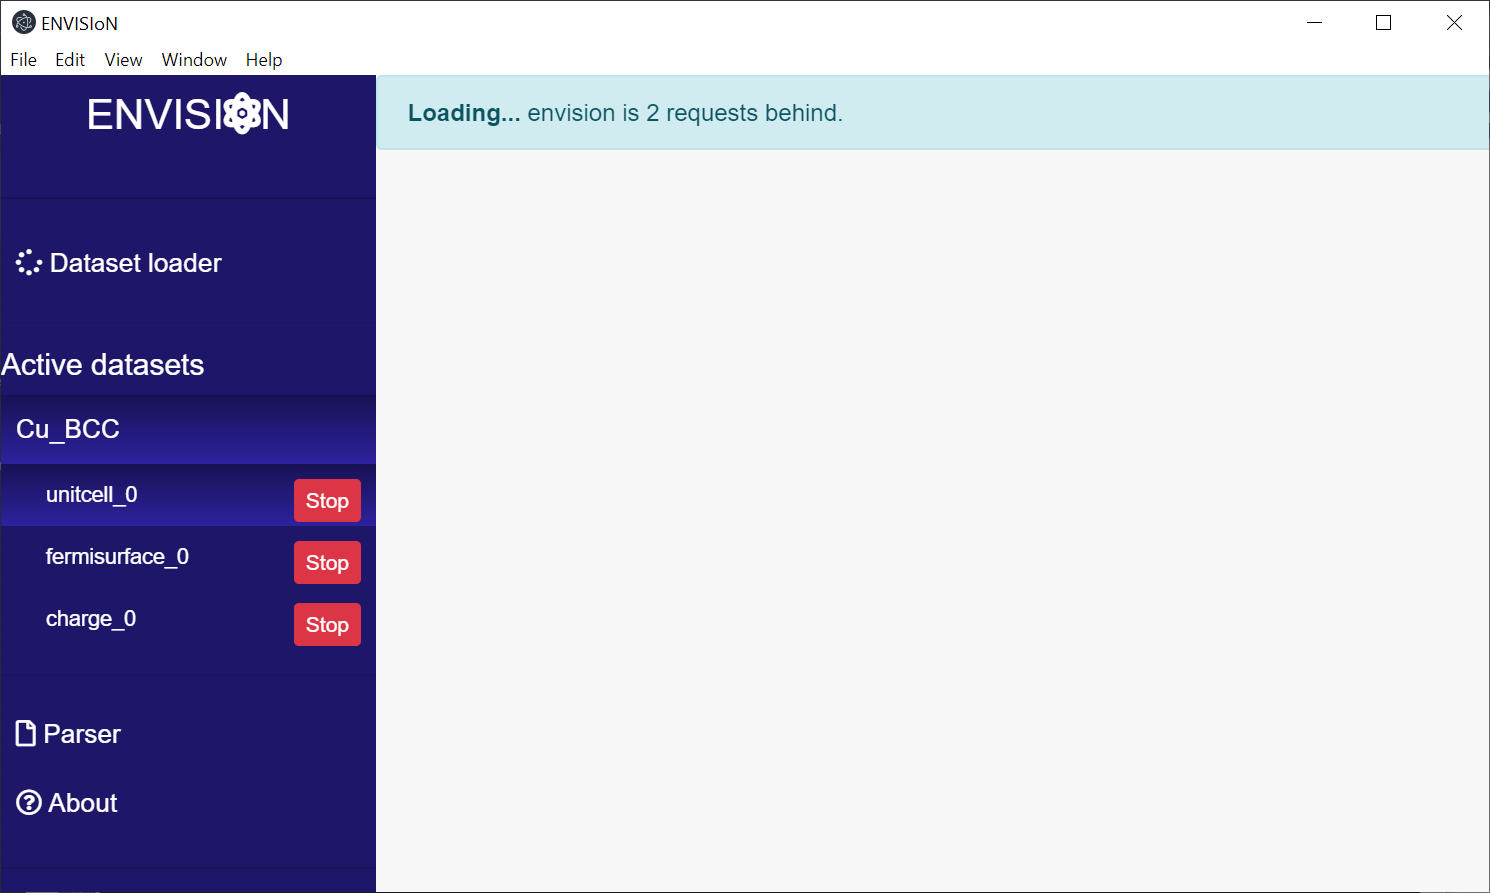
\includegraphics[scale = 0.45]{Images/EnvisionRequestsbehind.png}
    \caption{The pop up when ENVISIoN is a number of requests behind.}
    \label{fig:GUINotresponding}
\end{figure}

To recover from that ENVISIoN is a number of requests behind you can click on ``View'' in the upper menu and then ``Reload'' to reload the GUI. Then you need to start from the beginning and load the dataset once again.

If ENVISIoN is a number of request behind and the user continues to click around in the GUI and tries to load a new dataset or create a new visualisation the GUI will crash. If it does the following message box will pop up, see figure \ref{fig:GUIcrash}.

\begin{figure}[H]
    \centering
    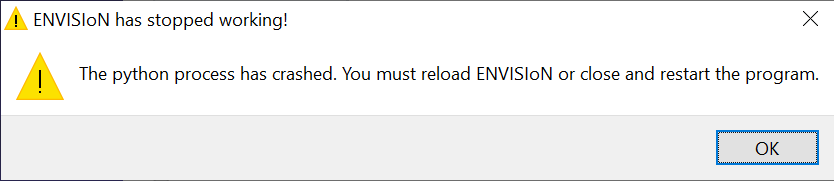
\includegraphics[scale = 0.55]{Images/Envisioncrashed.png}
    \caption{The message box when ENVISIoN crashes.}
    \label{fig:GUIcrash}
\end{figure}

To recover from that ENVISIoN crashes you can either reload the page as mentioned above, or just close the GUI window and restart ENVISIoN.

    \newpage
    \section{Common errors during installation}
\subsection{Qt}
Inviwo uses the graphics library Qt which isn't always installed properly. These instructions show how to download and install the latest version of Qt on Ubuntu 10.04 LTS. That is, in the moment of writing this user guide, version 5.12.3. 

To download the installation file into the \emph{~/Downloads} directory, simply execute the commands below.

\begin{lstlisting}[frame = single, breaklines=true]
    cd ~/Downloads
    wget http://download.qt.io/official_releases/qt/5.12/5.12.3/qt-opensource-linux-x64-5.12.3.run
    
    
    
\end{lstlisting}

When the installation file has finished downloading, the user won't have permission to run the file. To change permissions and run the file by executing the commands below and enter your superuser password immediately after.
\begin{lstlisting}[frame = single, breaklines=true]
    chmod +x qt-opensource-linux-x64-5.12.3.run
    sudo ./qt-opensource-linux-x64-5.12.3.run
\end{lstlisting}

An Qt installer is now shown on the screen. Notice that the manual installation will force a installation of the Qt editor as shown in step 6. The entire installation will occupy approximately 5.12 GB. Follow the instructions in figure \ref{fig:Qt} to complete the installation.

After the installation is done, the path to Qt needs to be added to the system. Add the necessary paths by executing the commands below.

\begin{lstlisting}[frame = single, breaklines=true]
    cd /usr/lib/x86_64-linux-gnu/qtchooser
    sudo echo "/opt/Qt5.12.3/5.12.3/gcc_64/bin" | sudo tee -a default.conf
    sudo echo "/opt/Qt5.12.3/5.12.3/gcc_64/lib" | sudo tee -a default.conf
\end{lstlisting}

The system is now ready for an Inviwo installation.

\begin{figure}[H]
    \centering
    \begin{subfigure}{0.32\linewidth}
        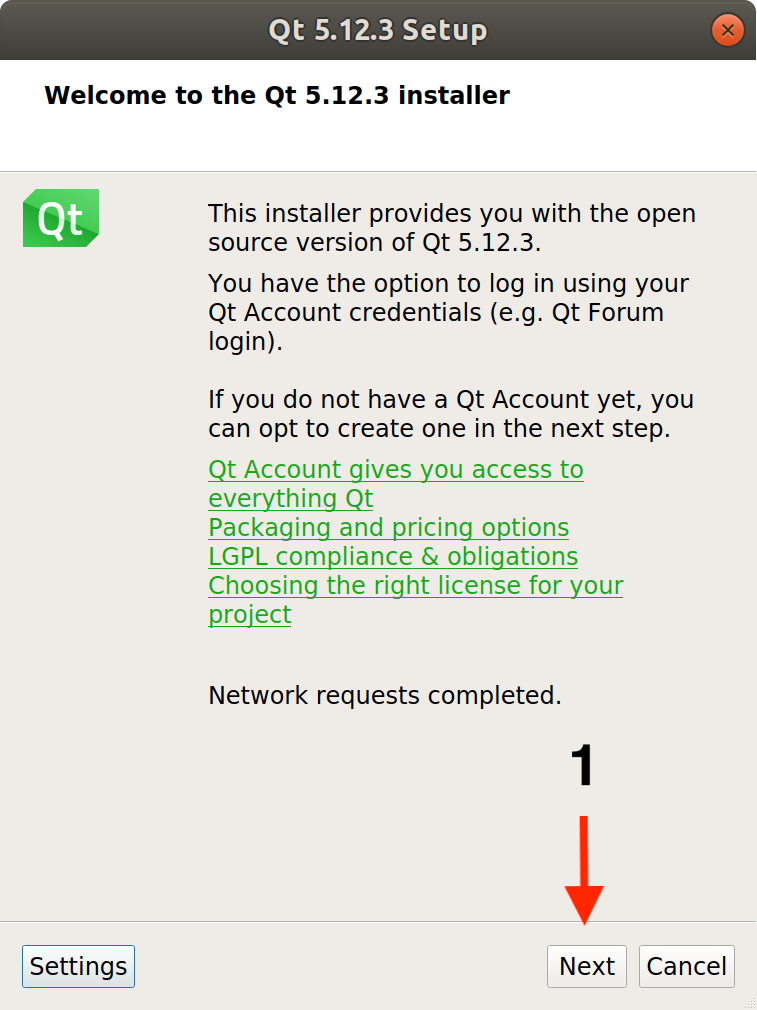
\includegraphics[width=1\textwidth]{images/Qt1.png}
    \end{subfigure}
    \begin{subfigure}{0.32\linewidth}
        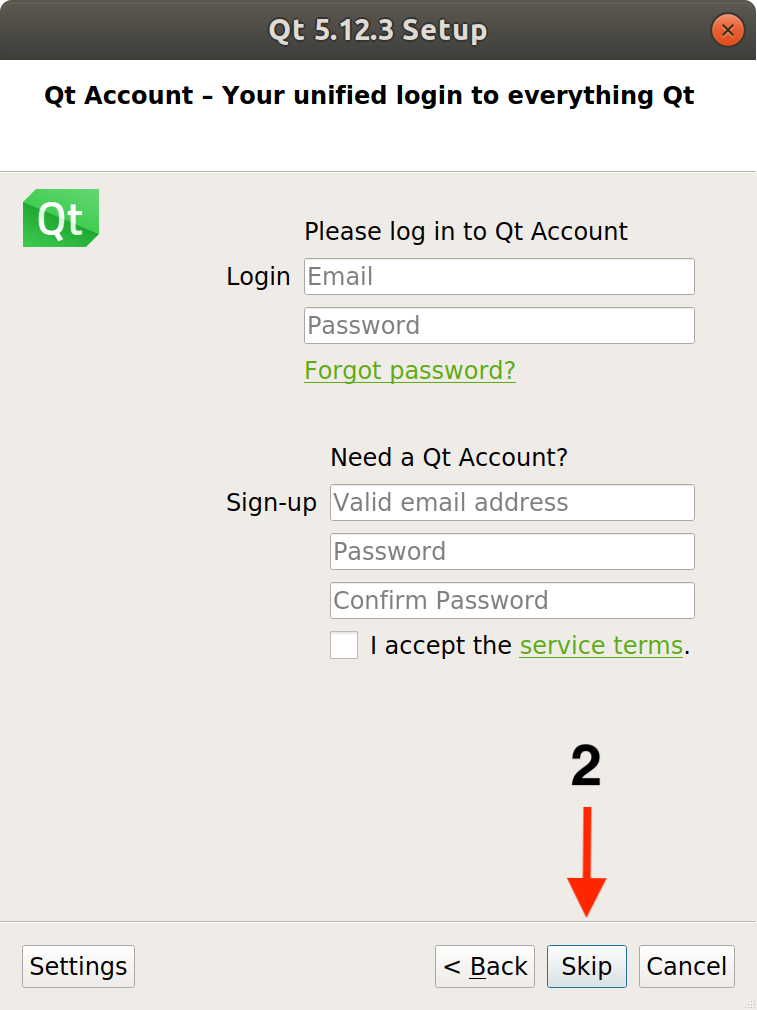
\includegraphics[width=1\textwidth]{images/Qt2.png}
    \end{subfigure}
    \begin{subfigure}{0.32\linewidth}
        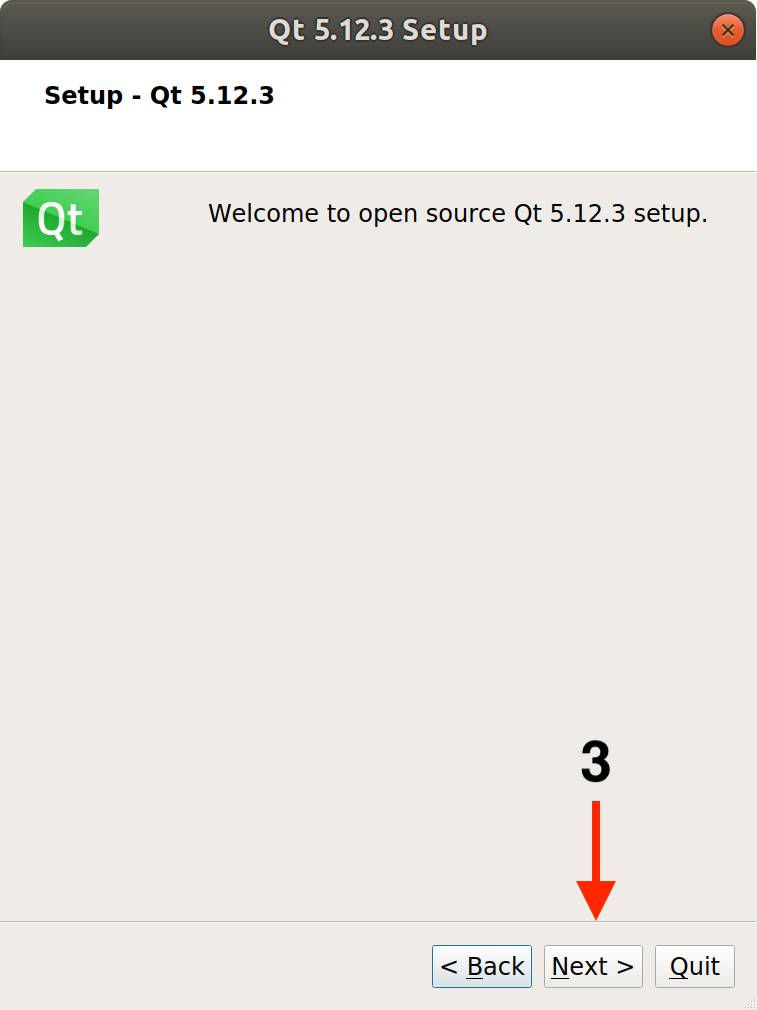
\includegraphics[width=1\textwidth]{images/Qt3.png}
    \end{subfigure}
    \begin{subfigure}{0.32\linewidth}
        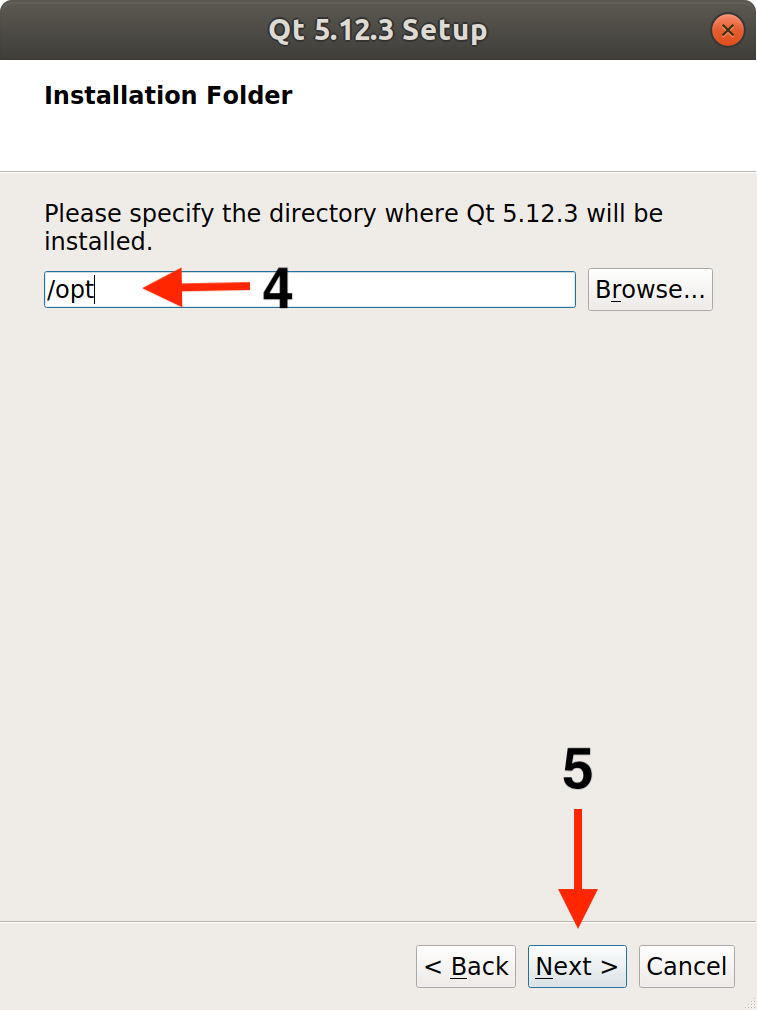
\includegraphics[width=1\textwidth]{images/Qt4.png}
    \end{subfigure}
    \begin{subfigure}{0.32\linewidth}
        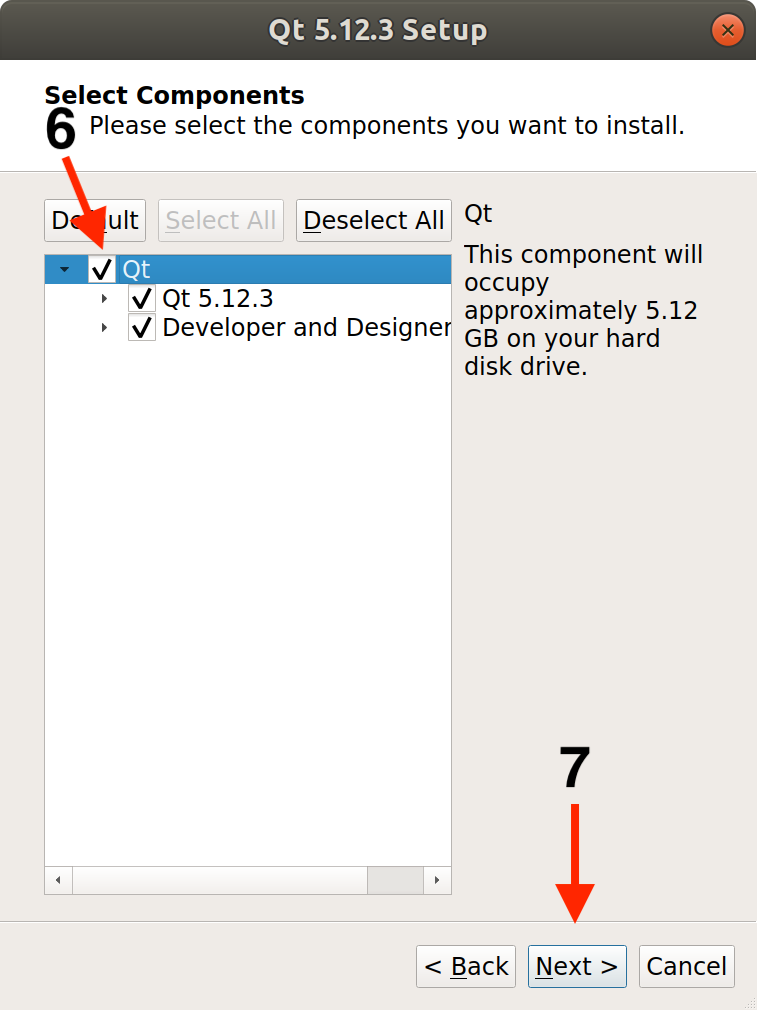
\includegraphics[width=1\textwidth]{images/Qt6.png}
    \end{subfigure}
    \begin{subfigure}{0.32\linewidth}
        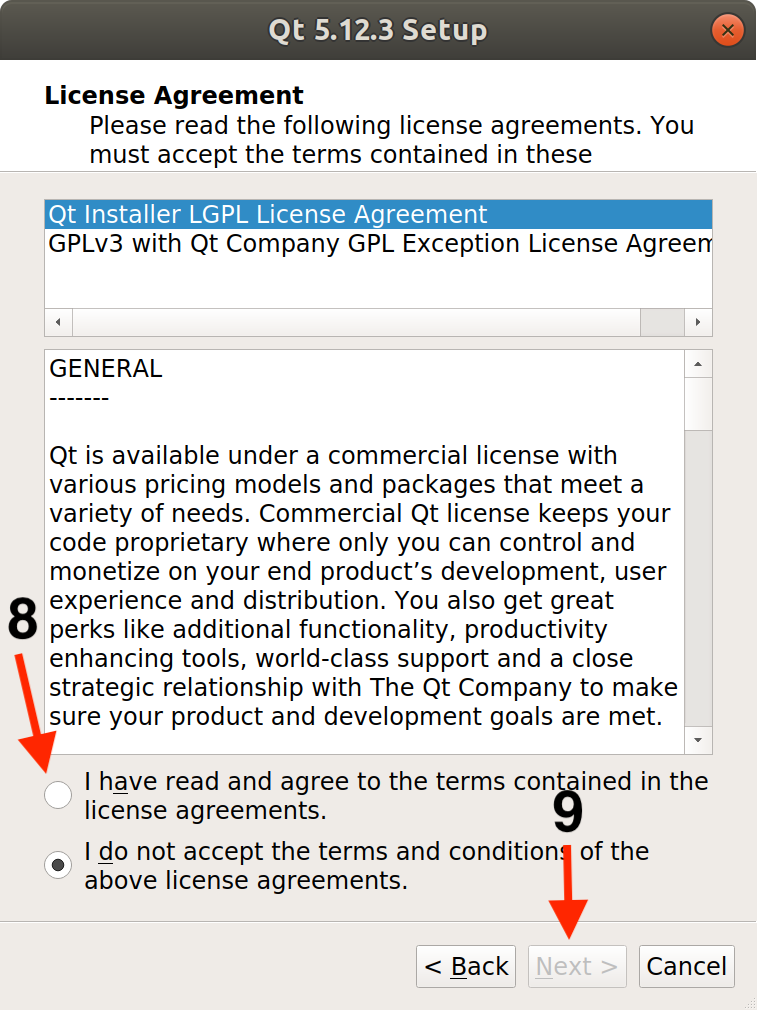
\includegraphics[width=1\textwidth]{images/Qt7.png}
    \end{subfigure}
    \begin{subfigure}{0.32\linewidth}
        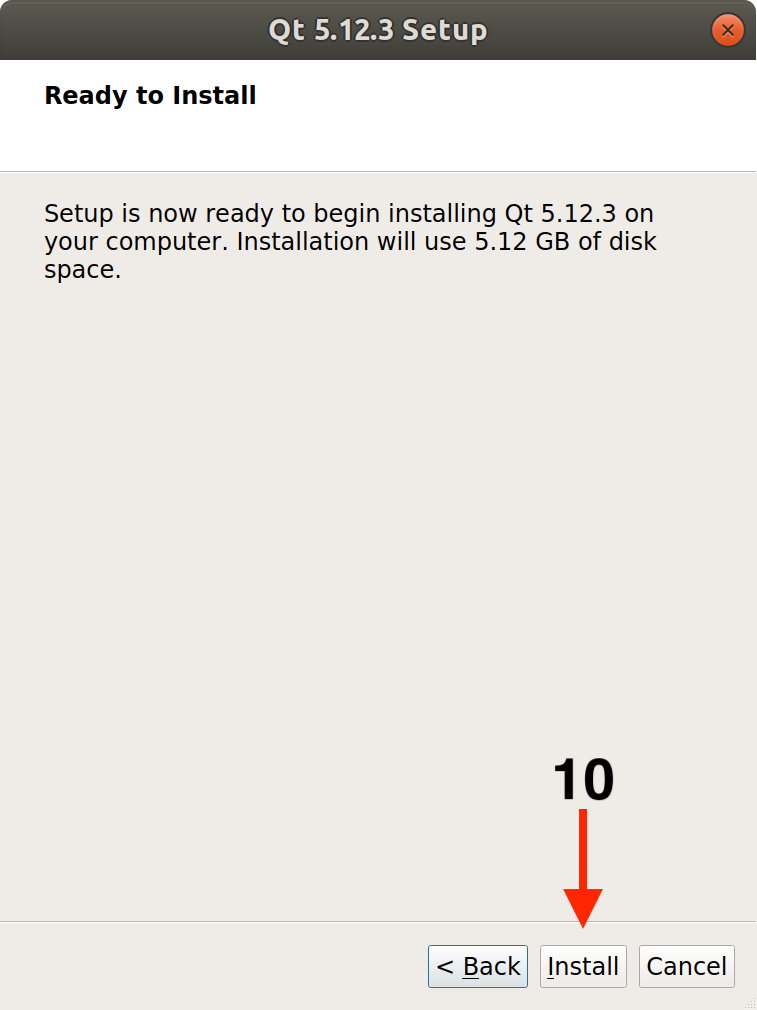
\includegraphics[width=1\textwidth]{images/Qt8.png}
    \end{subfigure}
    \caption{Instructions for installation of Qt 5.12.3.}
    \label{fig:Qt}
\end{figure}

    \newpage
    \begin{appendices}
        \section{Licens}
\label{ref:licens}
Copyright (c) 2021: Gabriel Anderberg, Kristoffer Gubberud Maras, Adam Engman, Joakim Stenborg, Didrik Axén \newline \newline
Copyright (c) 2020: Alexander Vevstad, Amanda Aasa, Amanda Svennblad, Daniel Thomas, Lina Larsson, Olav Berg

Redistribution and use in source and binary forms, with or without
modification, are permitted provided that the following conditions are met:

\begin{enumerate}
    \item Redistributions of source code must retain the above copyright notice, this list of conditions and the following disclaimer.
    \item Redistributions in binary form must reproduce the above copyright notice, this list of conditions and the following disclaimer in the documentation and/or other materials provided with the distribution.
\end{enumerate}

THIS SOFTWARE IS PROVIDED BY THE COPYRIGHT HOLDERS AND CONTRIBUTORS "AS IS" AND ANY EXPRESS OR IMPLIED WARRANTIES, INCLUDING,
BUT NOT LIMITED TO, THE IMPLIED WARRANTIES OF MERCHANTABILITY AND FITNESS FOR A PARTICULAR PURPOSE ARE DISCLAIMED. IN NO EVENT
SHALL THE COPYRIGHT OWNER OR CONTRIBUTORS BE LIABLE FOR ANY DIRECT, INDIRECT, INCIDENTAL, SPECIAL, EXEMPLARY, OR CONSEQUENTIAL
DAMAGES (INCLUDING, BUT NOT LIMITED TO, PROCUREMENT OF SUBSTITUTE GOODS OR SERVICES; LOSS OF USE, DATA, OR PROFITS; OR BUSINESS
INTERRUPTION) HOWEVER CAUSED AND ON ANY THEORY OF LIABILITY, WHETHER IN CONTRACT, STRICT LIABILITY, OR TORT (INCLUDING
NEGLIGENCE OR OTHERWISE) ARISING IN ANY WAY OUT OF THE USE OF THIS SOFTWARE, EVEN IF ADVISED OF THE POSSIBILITY OF SUCH DAMAGE.

        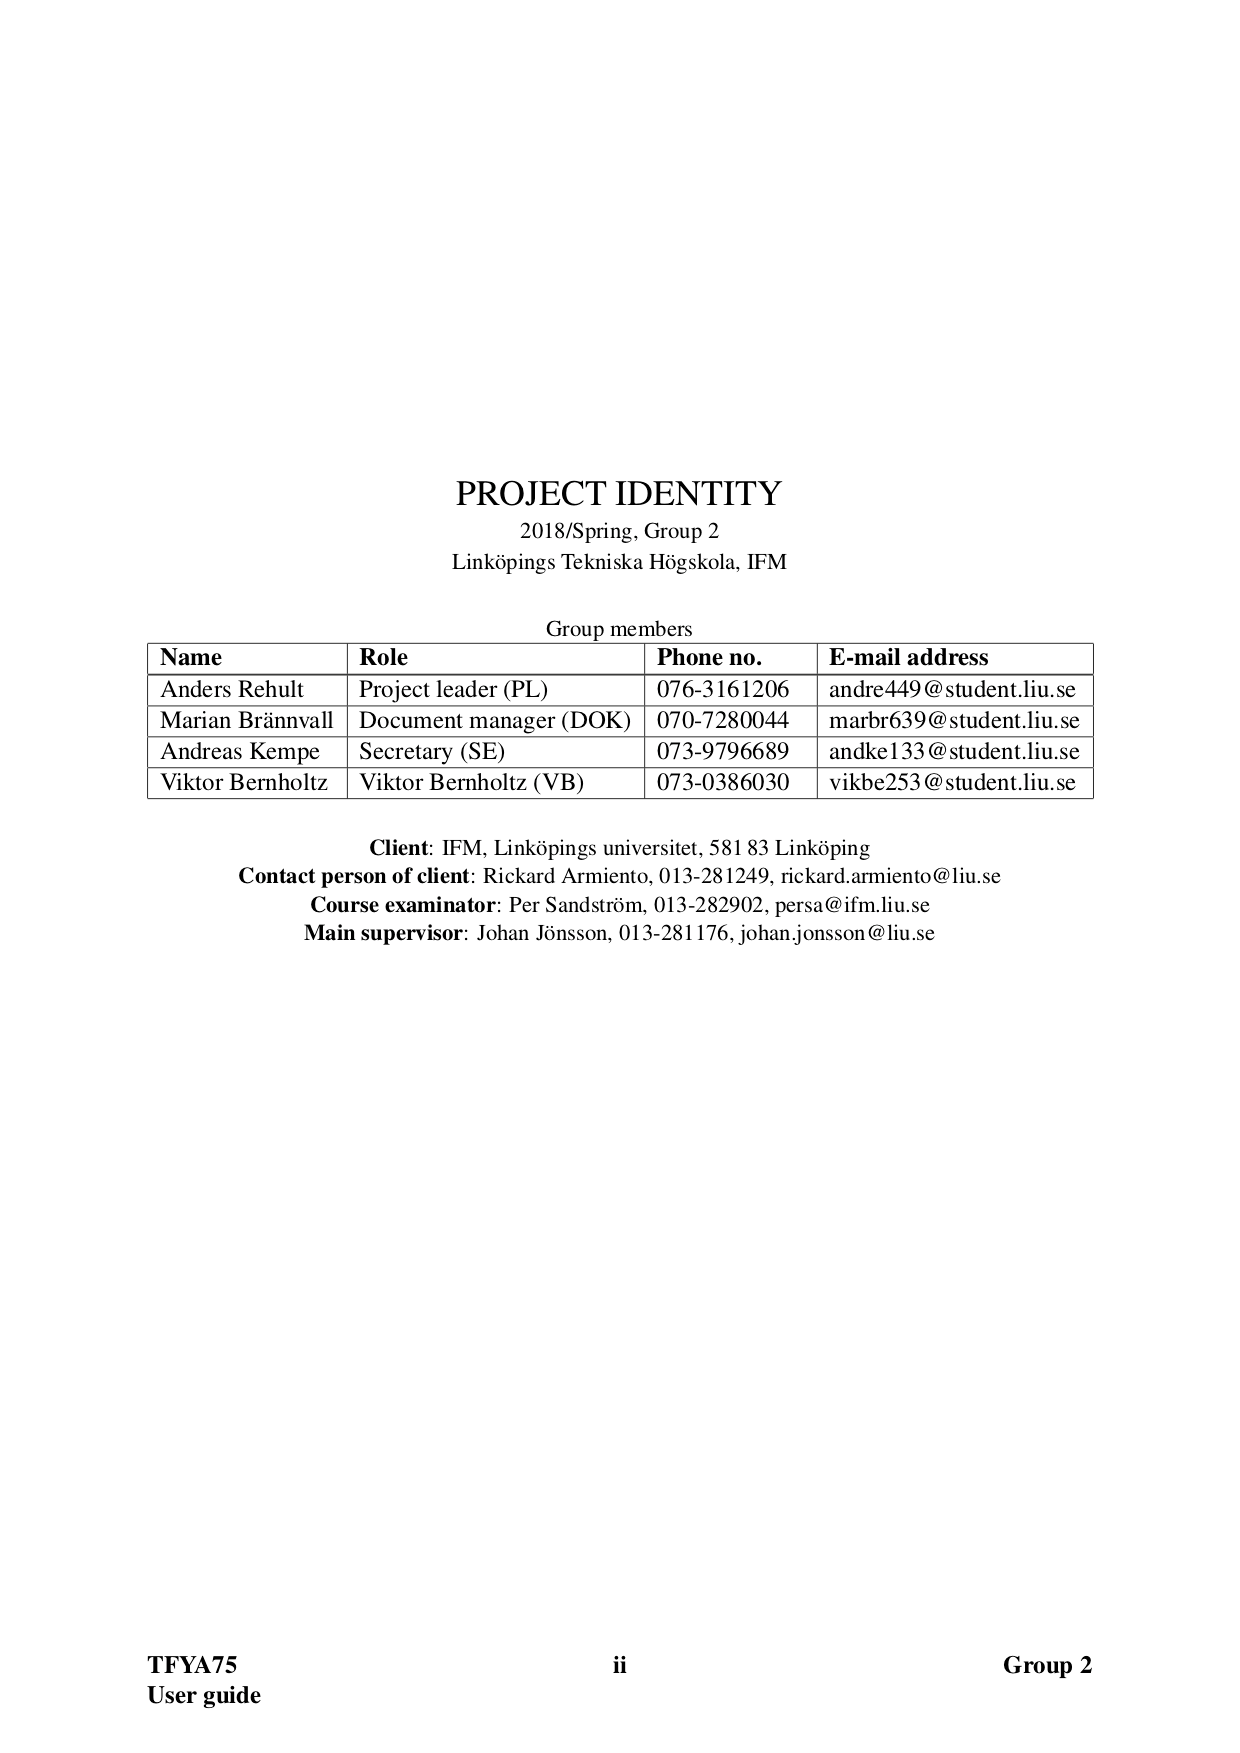
\includepdf[pages={1},offset= 0mm 0mm,pagecommand=\section{Projekt group 2018}\label{appendix:userGuide2018}\thispagestyle{empty}]{oldUserGuide.pdf}
        \includepdf[pages={2-}]{oldUserGuide.pdf}   
    \end{appendices}
\end{document}
